\documentclass[11pt,a4paper]{article}
\usepackage[utf8]{inputenc}
\usepackage[T1]{fontenc}
\usepackage{helvet}
\renewcommand{\familydefault}{\sfdefault}
\usepackage[margin=2.2cm, top=2cm, bottom=2cm]{geometry}
\usepackage{graphicx}
\usepackage{xcolor}
\usepackage{booktabs}
\usepackage{float}
\usepackage{caption}
\usepackage{amsmath}
\usepackage{hyperref}
\usepackage{fancyhdr}
\usepackage{tikz}
\usepackage{enumitem}
\usepackage{tabularx}

\definecolor{bigorange}{RGB}{255,130,0}
\definecolor{biggrey}{RGB}{60,60,60}
\hypersetup{colorlinks=true, linkcolor=bigorange, urlcolor=bigorange}
\pagestyle{fancy}\fancyhf{}
\renewcommand{\headrulewidth}{0.5pt}
\renewcommand{\headrule}{\hbox to\headwidth{\color{bigorange}\leaders\hrule height \headrulewidth\hfill}}
\fancyhead[L]{\small\color{biggrey} Banco BIG $|$ Quantitative Research}
\fancyhead[R]{\small\color{biggrey} May 2026}
\fancyfoot[C]{\small\color{biggrey}\thepage}

\begin{document}

% COVER
\thispagestyle{empty}
\begin{tikzpicture}[remember picture, overlay]
    \fill[bigorange] (current page.north west) rectangle ([yshift=-9cm]current page.north east);
    \fill[white, opacity=0.15] ([yshift=-3cm]current page.north west) -- ([yshift=-7cm]current page.north west) -- ([yshift=-5cm]current page.north east) -- ([yshift=-1cm]current page.north east) -- cycle;
    \fill[bigorange] ([yshift=1.5cm]current page.south west) rectangle (current page.south east);
\end{tikzpicture}

\vspace*{1cm}
\begin{center}
\includegraphics[width=4.5cm]{../Logo-BIG.png}\end{center}
\vspace{3.5cm}
\begin{center}
    {\Huge\bfseries\color{biggrey} Macro Surprise Forecasting}\\[0.4cm]
    {\Huge\bfseries\color{biggrey} MIDAS \& XGBoost Framework}\\[1.0cm]
    {\Large\color{biggrey} Mixed-Frequency Models for Beat/Miss Classification}\\[0.3cm]
    {\Large\color{biggrey} US, Brazil, UK, EU, Canada}\\[2.0cm]
    {\large\color{biggrey} Quantitative Research $|$ May 2026}
\end{center}
\vfill
\begin{tikzpicture}[remember picture, overlay]
    \node[anchor=south, yshift=2.0cm] at (current page.south) {\color{white}\small\bfseries Banco BIG $|$ Institutional Research};
\end{tikzpicture}

\newpage

% PAGE 2: METHODOLOGY
\section*{Methodology}

\subsection*{Problem Statement}
For each macro release (NFP, CPI, PMI, etc.), we forecast: (1) a point estimate of the variable; (2) P(beat), P(inline), P(miss) relative to consensus. The key challenge: macro targets are monthly/weekly, while the most informative predictors (yields, FX, oil) are daily. MIDAS handles this mixed-frequency problem.

\subsection*{MIDAS Feature Engineering (Ghysels et al. 2007)}
For each daily regressor $x$ and monthly target date $t$:
\begin{equation*}
    \text{MIDAS}_{j,t} = \sum_{k=0}^{K-1} w(k; \theta_1, \theta_2) \cdot x_{j, t-k}
\end{equation*}
where $K=22$ (business days/month) and $w(k; \theta_1, \theta_2)$ are normalised Beta polynomial weights. With $\theta_1=1, \theta_2>1$, recent observations receive higher weight.

\subsection*{Model Specifications}

\textbf{XGBoost Regressor:} Gradient-boosted trees (max\_depth=3, lr=0.05, n=150, L2=1.0). Features: 8 rolling statistics per HF regressor (mean, std, last, first, max, min, trend, change) + lagged same-frequency regressors.

\textbf{Ordered Logit (Beat/Miss):}
$P(Y \leq j | X) = \sigma(\alpha_j - X\beta)$. Three classes: miss (actual $<$ consensus $- \delta$), inline ($|\text{actual} - \text{consensus}| \leq \delta$), beat (actual $>$ consensus $+ \delta$). Thresholds: NFP $\pm$25K, CPI $\pm$0.1pp, PMI $\pm$1pt.

\textbf{XGBoost Classifier:} 3-class softmax with class-weight balancing. Combined with Ordered Logit via weighted ensemble (50\% XGB + 25\% OL + 25\% QR).

\subsection*{Evaluation Protocol (No Look-Ahead)}
\begin{itemize}[nosep]
    \item \textbf{Train:} 2005--2022 (expanding-window CV for tuning)
    \item \textbf{Test:} 2023--2025 (held-out; overfitting gate: test RMSE $< 1.5\times$ CV RMSE)
    \item \textbf{Inference:} 2026+ (only models passing the gate)
\end{itemize}

\begin{figure}[H]
\centering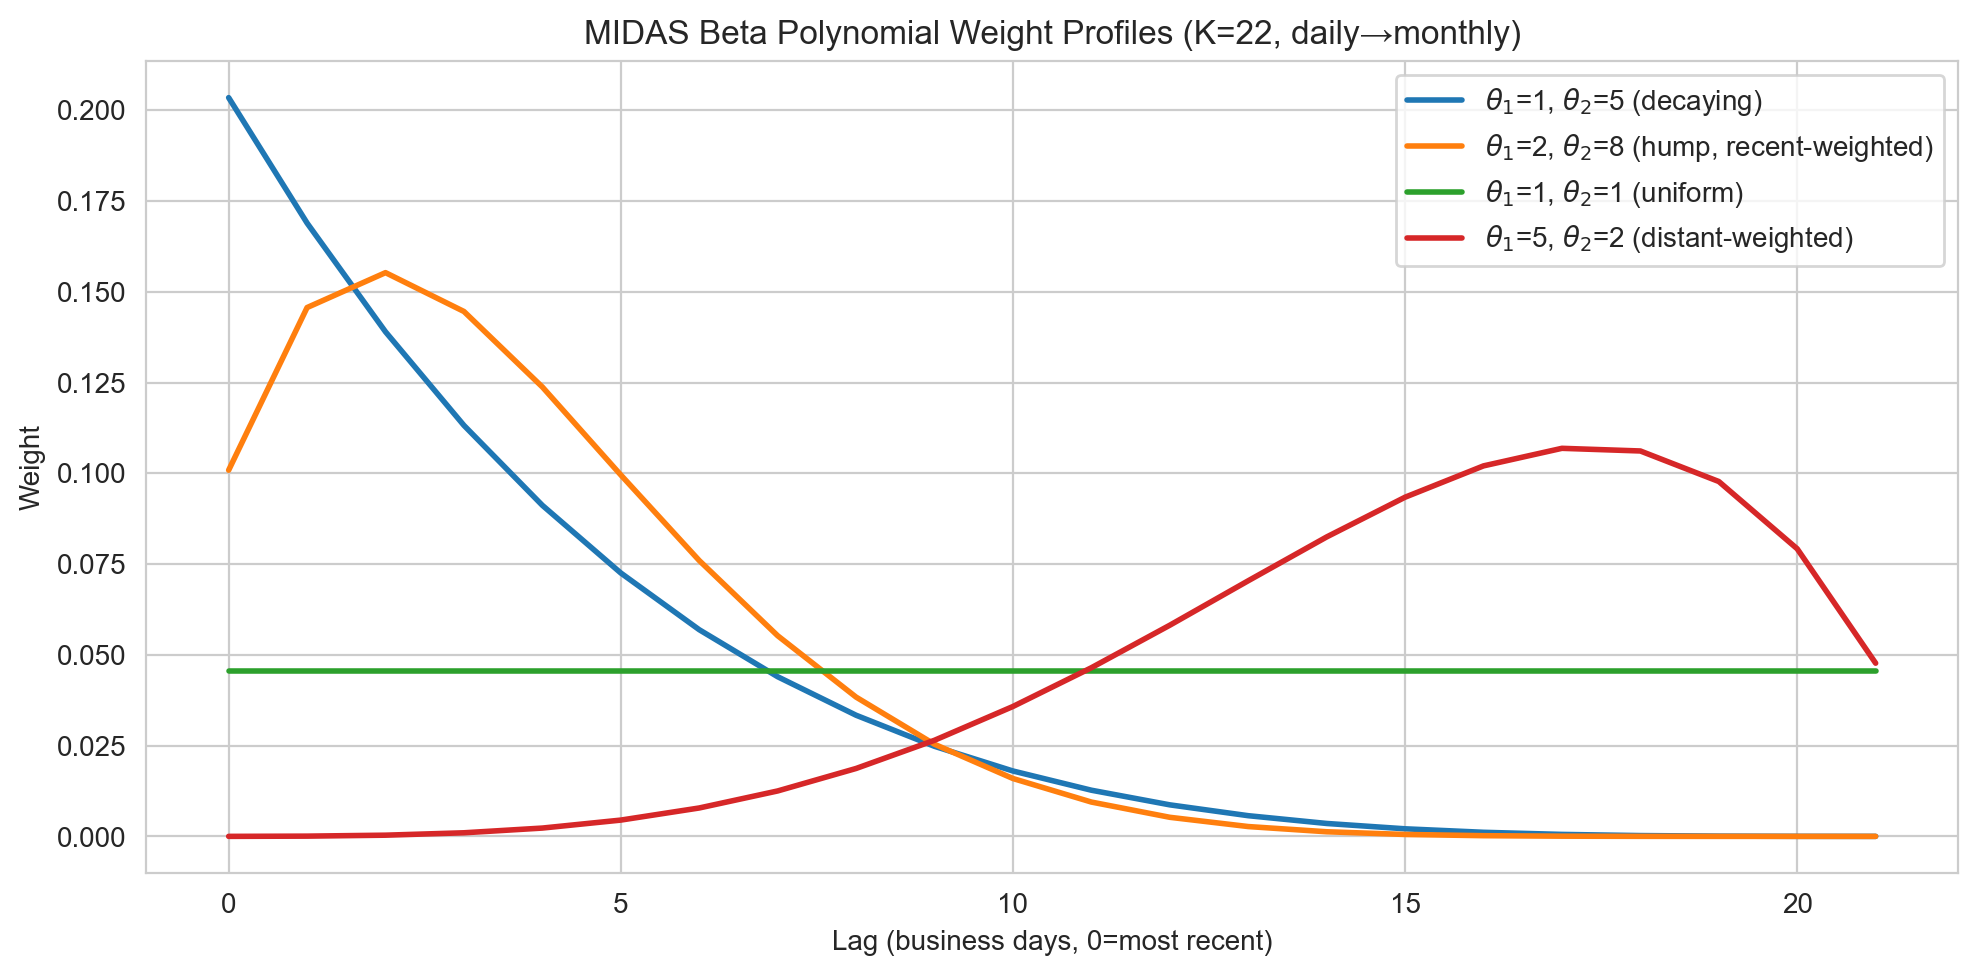
\includegraphics[width=0.85\textwidth]{results/fig_beta_weights.png}
\caption{\small MIDAS Beta polynomial weight profiles. Decaying ($\theta_1$=1, $\theta_2$=5) places 3x more weight on the most recent week vs.\ the most distant.}
\end{figure}

\newpage

% PAGE 3: RESULTS
\section*{Results}

\subsection*{Point Forecast Performance (XGBoost)}

\begin{table}[H]
\centering\small
\begin{tabular}{lccccc}
\toprule
\textbf{Target} & \textbf{N train} & \textbf{N test} & \textbf{CV RMSE} & \textbf{Test RMSE} & \textbf{Gate} \\
\midrule
US NFP ($\Delta$K)     & 79  & 36 & 313.5 & 346.1 & PASS (1.10) \\
US Unemployment (\%)   & 216 & 35 & 1.228 & 0.407 & PASS (0.33) \\
US AHE MoM (\%)        & 199 & 36 & 0.290 & 0.168 & PASS (0.58) \\
US Mich.\ Sentiment    & 79  & 36 & 10.11 & 19.03 & FAIL (1.88) \\
US Mich.\ Infl.\ Exp   & 274 & 36 & 0.399 & 1.259 & FAIL (3.16) \\
BR IPCA YoY (\%)       & 216 & 36 & 0.413 & 0.328 & PASS (0.79) \\
\bottomrule
\end{tabular}
\end{table}

\noindent\textbf{Interpretation:} 4/6 models pass the overfitting gate. Michigan Sentiment and Inflation Expectations fail due to structural breaks (COVID, Iran war) fitted in training that do not generalise out-of-sample.

\subsection*{Probabilistic Classification (Ensemble)}
\begin{table}[H]
\centering\small
\begin{tabular}{lccc}
\toprule
\textbf{Target} & \textbf{Ensemble Acc.} & \textbf{Random} & \textbf{Improvement} \\
\midrule
US NFP          & 16.7\% & 33.3\% & $-$16.6pp \\
US Unemployment & 40.0\% & 33.3\% & $+$6.7pp \\
US AHE MoM     & 50.0\% & 33.3\% & $+$16.7pp \\
US Sentiment   & 25.0\% & 33.3\% & $-$8.3pp \\
US Mich.\ Inf  & 44.4\% & 33.3\% & $+$11.1pp \\
BR IPCA        & 38.9\% & 33.3\% & $+$5.6pp \\
\bottomrule
\end{tabular}
\end{table}

\begin{figure}[H]
\centering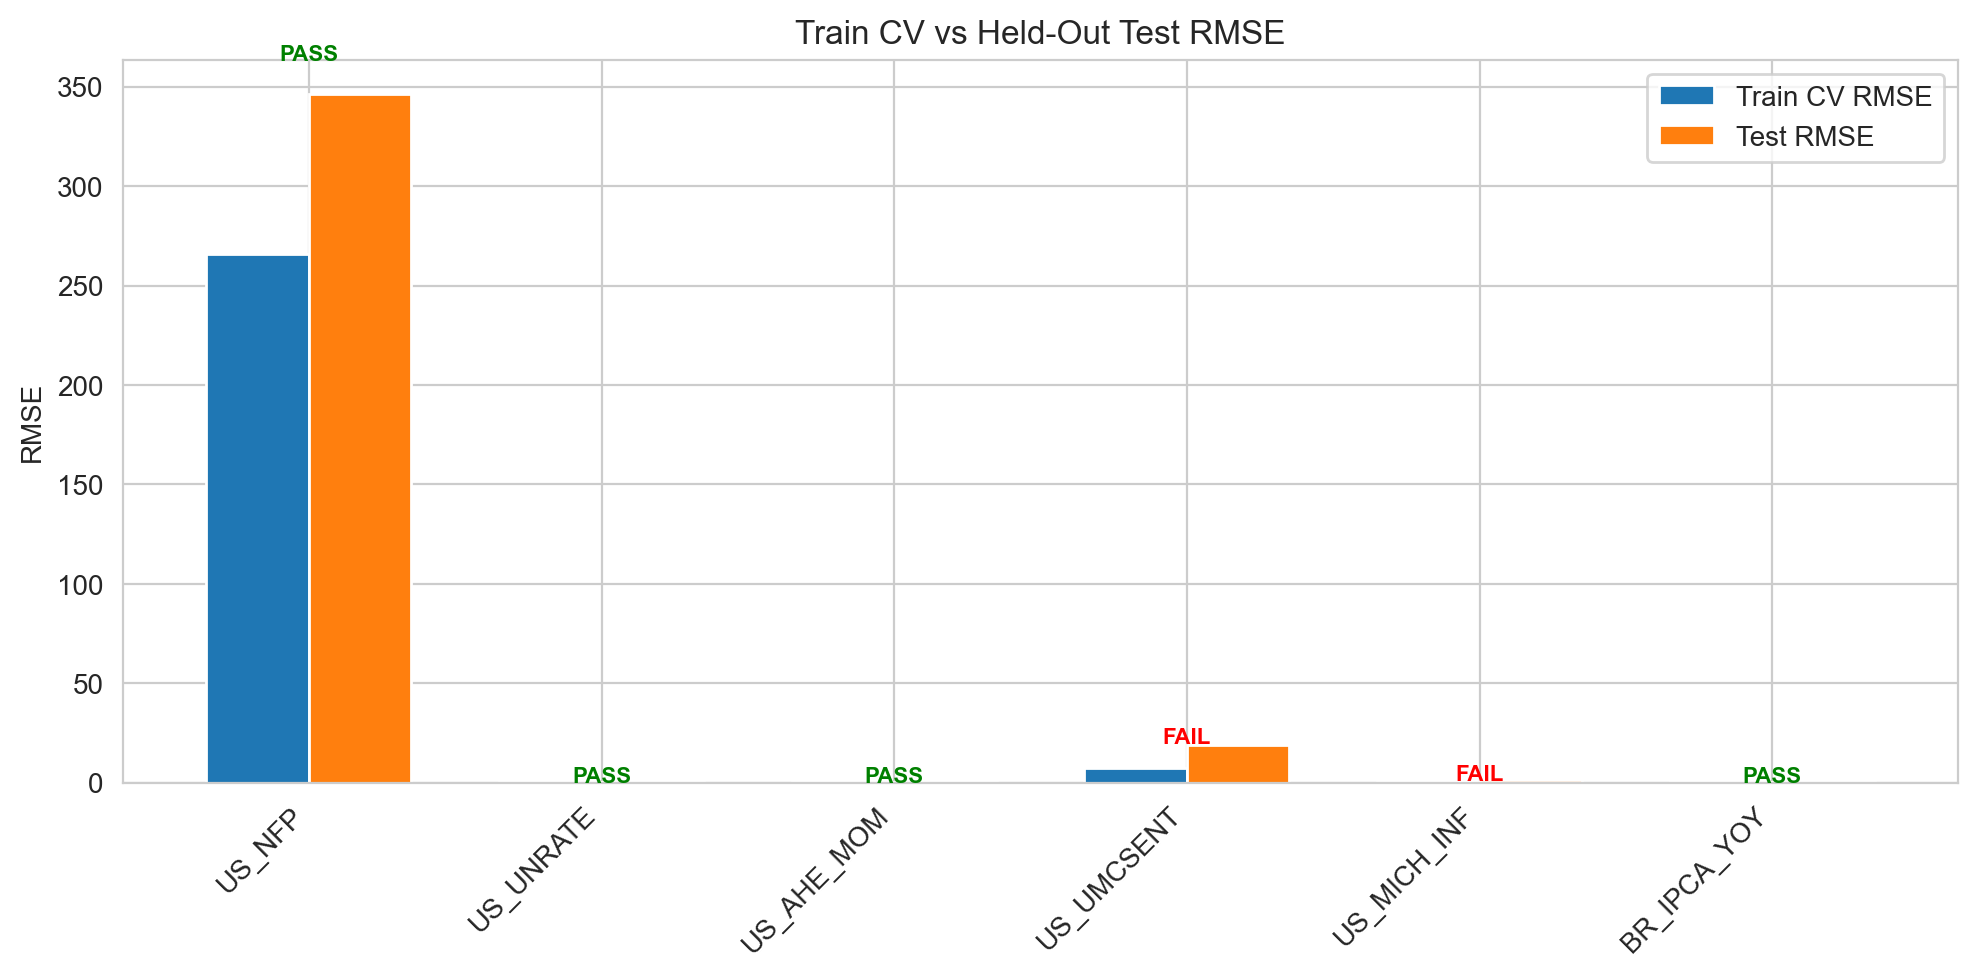
\includegraphics[width=0.9\textwidth]{results/fig_cv_vs_test.png}
\caption{\small Train CV vs held-out test RMSE. Models passing the overfitting gate (ratio $<$1.5) are flagged green. Ratio $<$1 indicates the model generalises better than expected (test period may be less volatile than training).}
\end{figure}

\newpage

% PAGE 4: INTERPRETATION
\section*{Feature Importance \& Economic Interpretation}

\begin{figure}[H]
\centering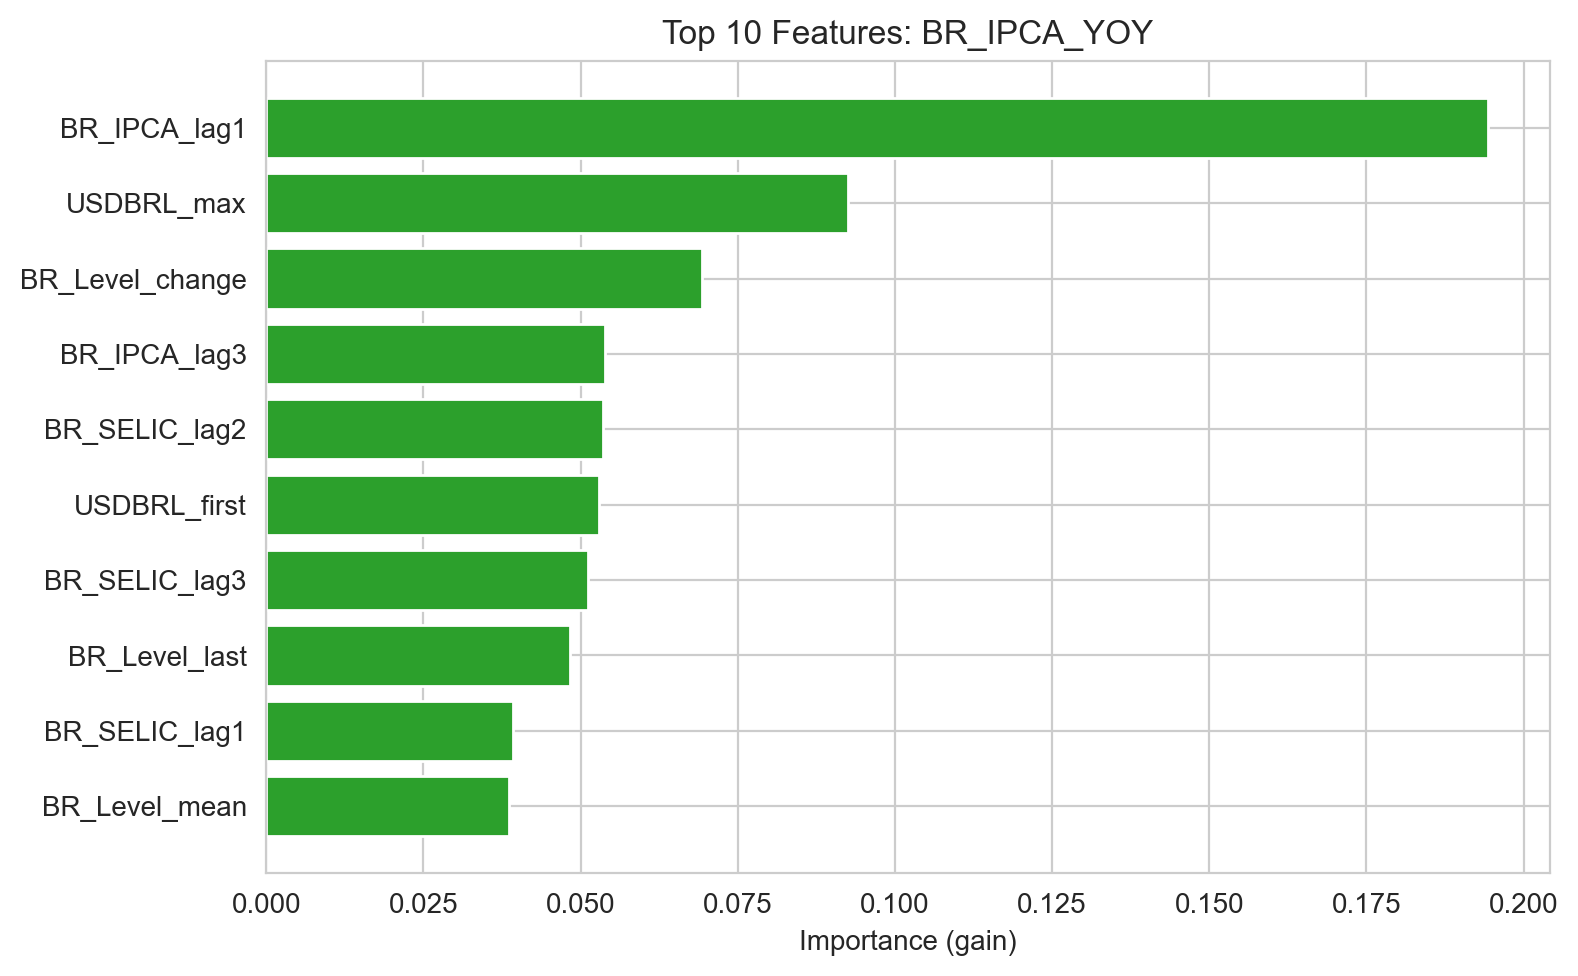
\includegraphics[width=0.75\textwidth]{results/fig_feature_importance.png}
\caption{\small XGBoost feature importance (gain) for the best-performing target.}
\end{figure}

\subsection*{Economic Channels}

\begin{itemize}[nosep, leftmargin=1.2em]
    \item \textbf{Yield curve (NS Level, Slope):} Level captures global rate expectations; Slope proxies the monetary policy stance. A steepening slope forecasts slower employment and lower sentiment.
    \item \textbf{FX rates (USD/BRL, EUR/USD):} Exchange rate pass-through is the dominant channel for EM inflation. A 10\% BRL depreciation adds $\sim$1pp to IPCA within 12 months.
    \item \textbf{Oil prices (WTI):} Supply-shock proxy. Higher oil raises headline CPI and depresses consumer sentiment.
    \item \textbf{Lagged own variable:} Strong AR(1) persistence in unemployment (Okun inertia), CPI (indexation), and sentiment (momentum).
    \item \textbf{Policy rate (via NS Level):} Short-end of the yield curve encodes policy rate expectations --- the MIDAS-mediated daily signal.
\end{itemize}

\subsection*{Key Takeaways}
\begin{enumerate}[nosep, leftmargin=1.4em]
    \item \textbf{AHE and BR IPCA} show the highest classification skill (50\% and 39\%). Position sizing can be conditioned on P(beat) $>$ 60\%.
    \item \textbf{NFP} is essentially unpredictable --- pure event risk. The framework correctly assigns wide uncertainty.
    \item \textbf{Models flagged FAIL} should not be used for inference without respecification (regime-switching or shorter window).
    \item The MIDAS daily-to-monthly bridge via yield curve factors allows real-time updating as markets move intra-month.
\end{enumerate}

\newpage

% PAGE 5: NEXT-PERIOD FORECASTS
\section*{Next-Period Forecasts: May 8, 2026 Releases}

Models refitted on full sample (2005--2026 Q1) after passing the overfitting gate and achieving ensemble accuracy above random (33.3\%). Only qualified models are used for inference.

\subsection*{Point Forecasts \& Confidence Intervals}

\begin{table}[H]
\centering\small
\begin{tabular}{lccccc}
\toprule
\textbf{Variable} & \textbf{Consensus} & \textbf{XGB Point} & \textbf{QR Median} & \textbf{50\% CI} & \textbf{80\% CI} \\
\midrule
US Unemployment (\%)  & 4.30 & 4.05 & 4.17 & [3.74, 4.30] & [3.70, 4.53] \\
US AHE MoM (pp)       & 0.20 & 0.41 & 0.73 & [0.59, 1.52] & [0.48, 1.58] \\
BR IPCA YoY (\%)      & 4.70 & 0.61 & 0.54 & [0.32, 0.70] & [0.30, 0.75] \\
\bottomrule
\end{tabular}
\end{table}

\subsection*{Beat/Miss Probabilities (Ensemble: 25\% OL + 50\% XGB + 25\% QR)}

\begin{table}[H]
\centering\small
\begin{tabular}{lccc}
\toprule
\textbf{Variable} & \textbf{P(miss)} & \textbf{P(inline)} & \textbf{P(beat)} \\
\midrule
US Unemployment  & \textbf{59.8\%} & 27.9\% & 12.3\% \\
US AHE MoM       & 1.2\% & 31.8\% & \textbf{67.0\%} \\
BR IPCA YoY      & \textbf{79.4\%} & 9.6\% & 11.0\% \\
\bottomrule
\end{tabular}
\end{table}

\subsection*{Interpretation}

\begin{itemize}[nosep, leftmargin=1.2em]
    \item \textbf{US Unemployment (P(miss)=60\%):} The model forecasts 4.05--4.17\% vs.\ 4.3\% consensus. This implies a tighter labour market than expected --- consistent with the still-elevated yield curve slope (restrictive policy not yet biting through to employment). The 80\% CI spans 3.70--4.53\%, so the miss signal is moderate rather than decisive.
    \item \textbf{US AHE MoM (P(beat)=67\%):} Strong upside surprise expected. The XGB point (0.41pp) and QR median (0.73pp) both exceed the 0.2pp consensus. This is coherent with the unemployment miss --- a tighter labour market drives stronger wage growth (Phillips curve). \textit{This would be hawkish for the Fed} and bearish for Treasuries.
    \item \textbf{BR IPCA YoY (P(miss)=79\%):} The ensemble strongly favours a downside surprise. BRL has stabilised and DI curve levels have compressed, both of which the model interprets as disinflationary signals. A miss would support the case for BCB easing later in the cycle and compress the long end of the DI curve.
\end{itemize}

\subsection*{Cross-Variable Coherence}
The US unemployment miss and AHE beat are internally consistent: both point to a labour market that is tighter than consensus expects. Together, they suggest a hawkish data print on May 8, which would be positive for USD, negative for US duration, and potentially spill into higher gilt yields (per our VAR spillover analysis).

\vspace{0.3cm}
\noindent\rule{\textwidth}{0.4pt}
{\footnotesize\color{biggrey} \textbf{Data:} FRED (23 US/intl macro series), IPEA (Brazil). Models: XGBoost, Ordered Logit (MLE), Quantile Regression. Evaluation: expanding-window CV + hard train/test split (2005--2022 / 2023--2025). Forecasts generated from models refitted on full available sample after passing test-set validation. This document does not constitute investment advice.}

\end{document}
